\documentclass[11pt]{article}
\usepackage{geometry}
\usepackage[colorlinks]{hyperref}
\usepackage{graphicx}
\usepackage{mathpazo}
\usepackage{epstopdf}
\usepackage[parfill]{parskip}
\usepackage{fancyvrb}
\usepackage{roundbox}

\makeatletter
\let \@sverbatim \@verbatim
\def \@verbatim {\@sverbatim \verbatimplus}
{\catcode`'=13 \gdef \verbatimplus{\catcode`'=13 \chardef '=13 }} 
\makeatother

\newcommand{\R}{\textsf{R}}

\begin{document}

\textbf{CVEN 4333, Spring 2010, Assignment \#12 Solutions}

\begin{enumerate}

\item Book problem 12.1

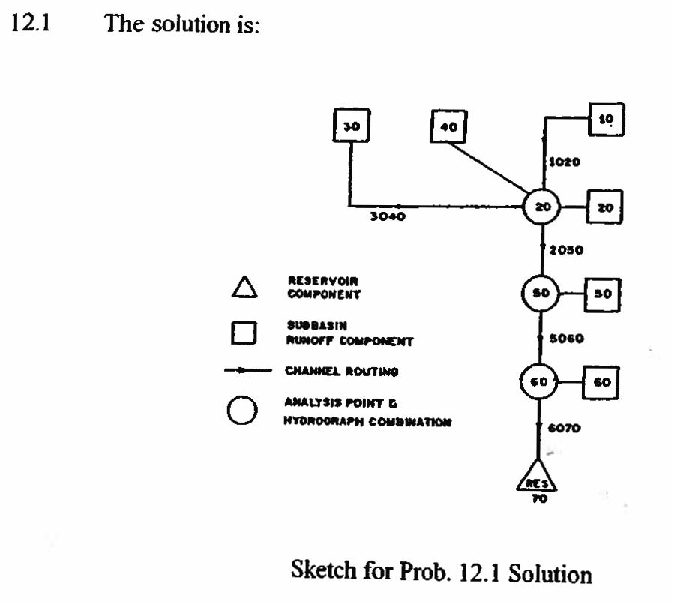
\includegraphics{12-1.pdf}

\clearpage
\item Book problem 12-5

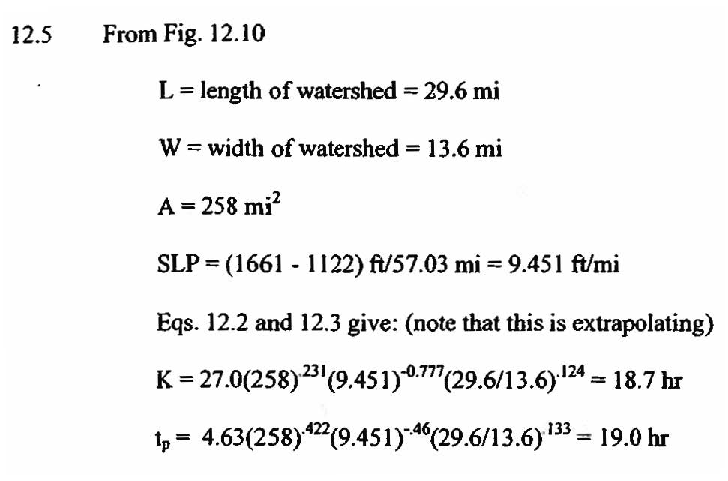
\includegraphics{12-5a.pdf}

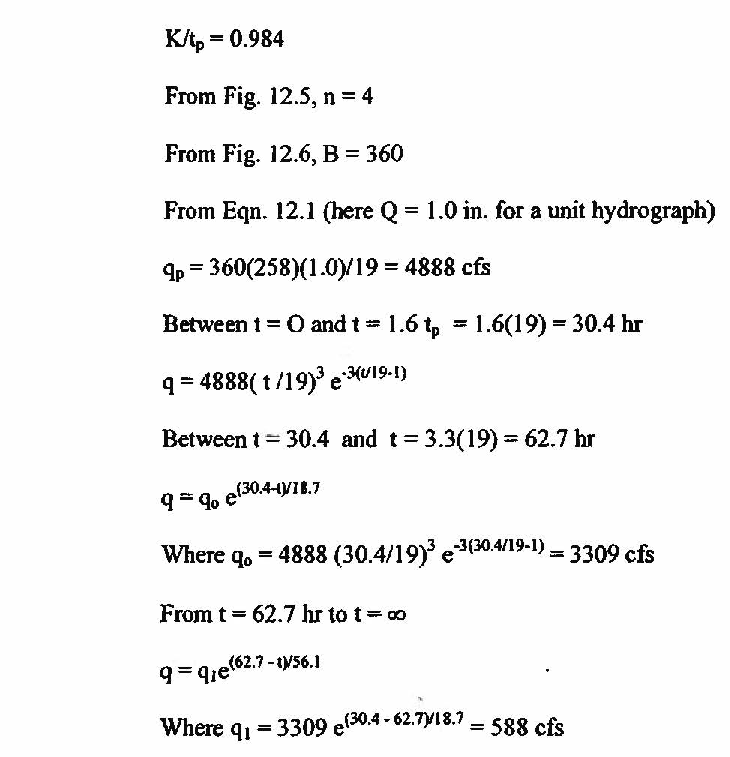
\includegraphics{12-5b.pdf}

\item Book problem 12-11

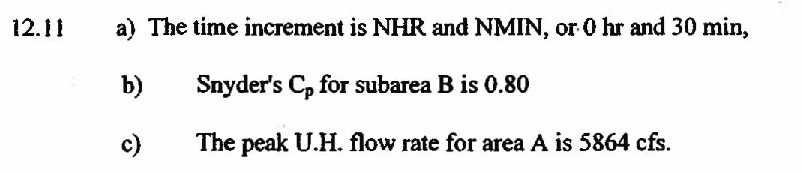
\includegraphics{12-11a.pdf}

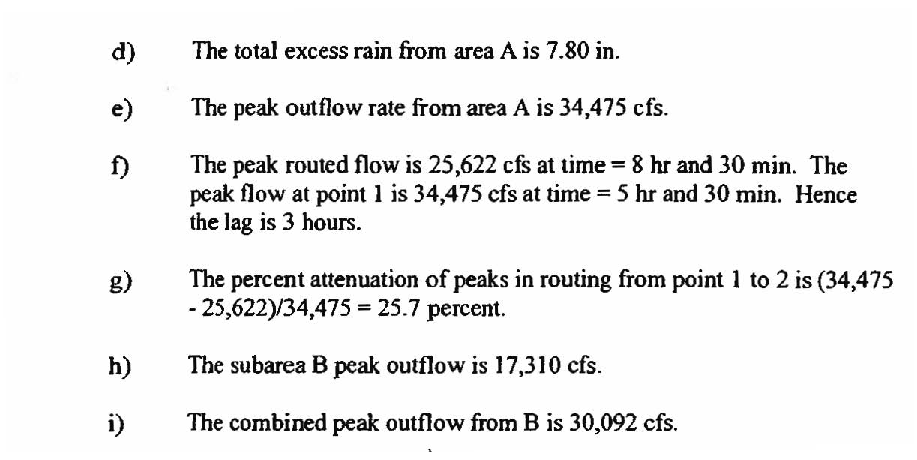
\includegraphics{12-11b.pdf}

\item Book problem 12-16 (Explain which equations you would use and outline how you would solve them. No need to do all the calculations)

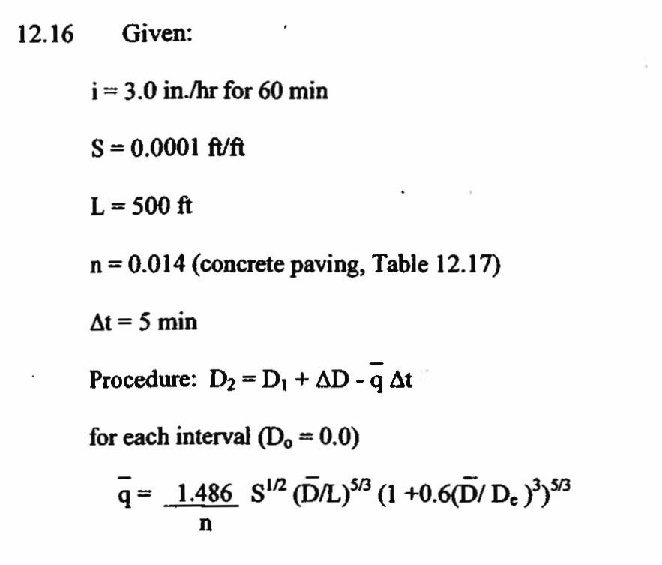
\includegraphics{12-16a.pdf}

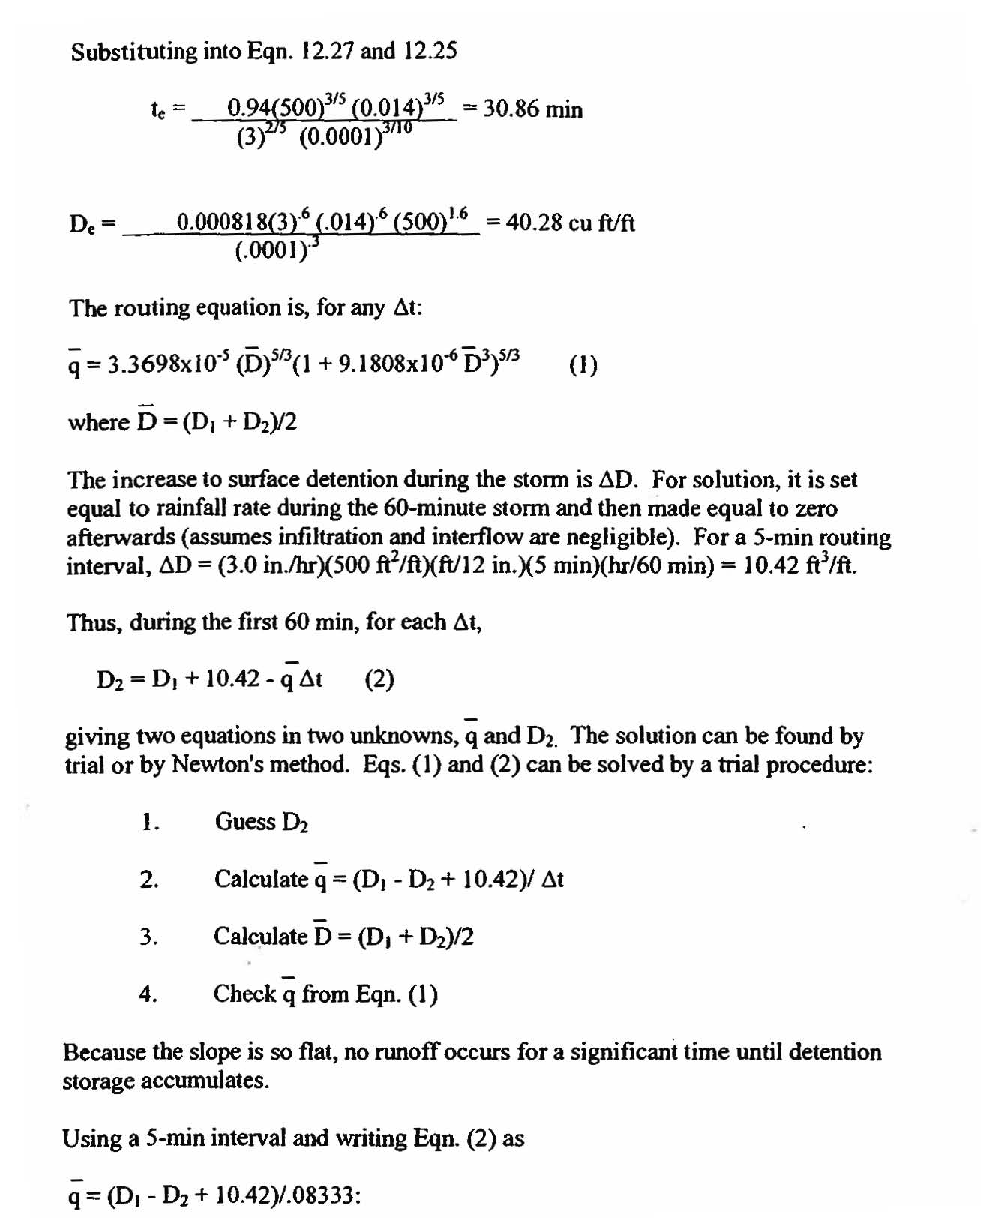
\includegraphics{12-16b.pdf}

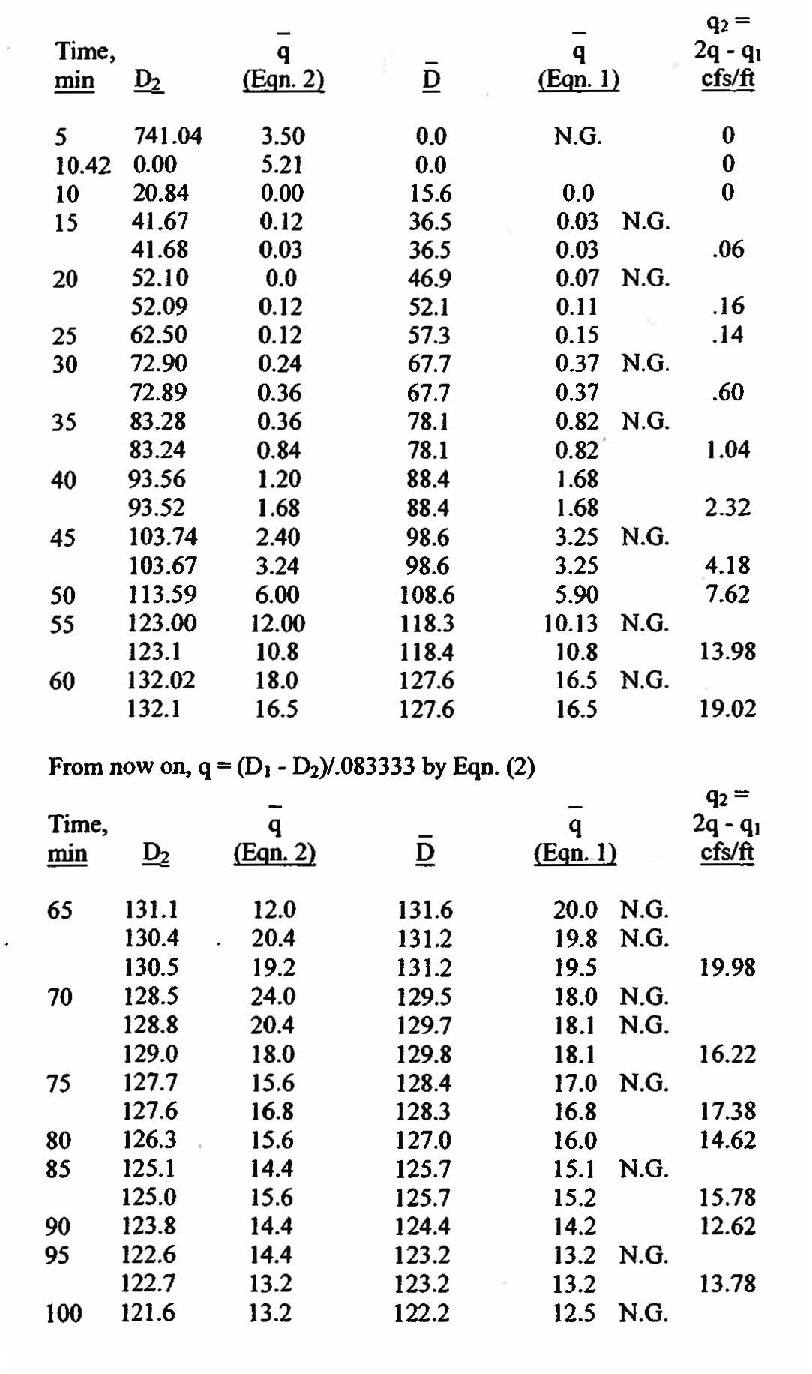
\includegraphics{12-16c.pdf}

\item Discuss in detail the SWM-IV model.
\begin{enumerate}
\item What processes does it simulate?
\item What equations are used for each process? Write them down and discuss.
\item Does this model need to be explicitly calibrated and if so how?
\end{enumerate}

\item Data analysis is an integral part of Hydrology. This semester we
primarily used R for data analysis though is is one of many tools we
could have used.   Investigate the statistical/numerical programs SAS,
SPSS, IDL, Matlab, R and Excel.  What are the pros/cons of each of
these pieces of software?  (Try to avoid "Sales pitches" and look for
intelligent criticisms)

\end{enumerate}
\end{document}  







